% ============================================================================
% ACM e-Energy — figures F7 / F8 for the results section.
% Include from the paper with:  % ============================================================================
% ACM e-Energy — figures F7 / F8 for the results section.
% Include from the paper with:  % ============================================================================
% ACM e-Energy — figures F7 / F8 for the results section.
% Include from the paper with:  % ============================================================================
% ACM e-Energy — figures F7 / F8 for the results section.
% Include from the paper with:  \input{f7_f8_figures}
% Requires: \usepackage{graphicx}
%
% Generated by:
%   python -m experiments.paper_figures.make_paper_figures \
%       --runs <runs-root> --out experiments/figures
% <runs-root> layout: <root>/<regime>/<scenario>/<run_id>/result.json
% Figures are vector PDF (fonts embedded) with SVG + 600 dpi PNG previews.
% ACM convention: figure captions go BELOW the figure.
%
% Self-contained: the F7 PDF is committed at paper/figures/. Compile from the
% paper directory (\graphicspath resolves both locations), or drop the PDF next
% to your main .tex.
% ============================================================================

\graphicspath{{figures/}{../experiments/figures/}}

% ----------------------------------------------------------------------------
% F7 — cost vs. service by pricing regime  (full width, two-column layout)
% ----------------------------------------------------------------------------
\begin{figure*}[t]
  \centering
  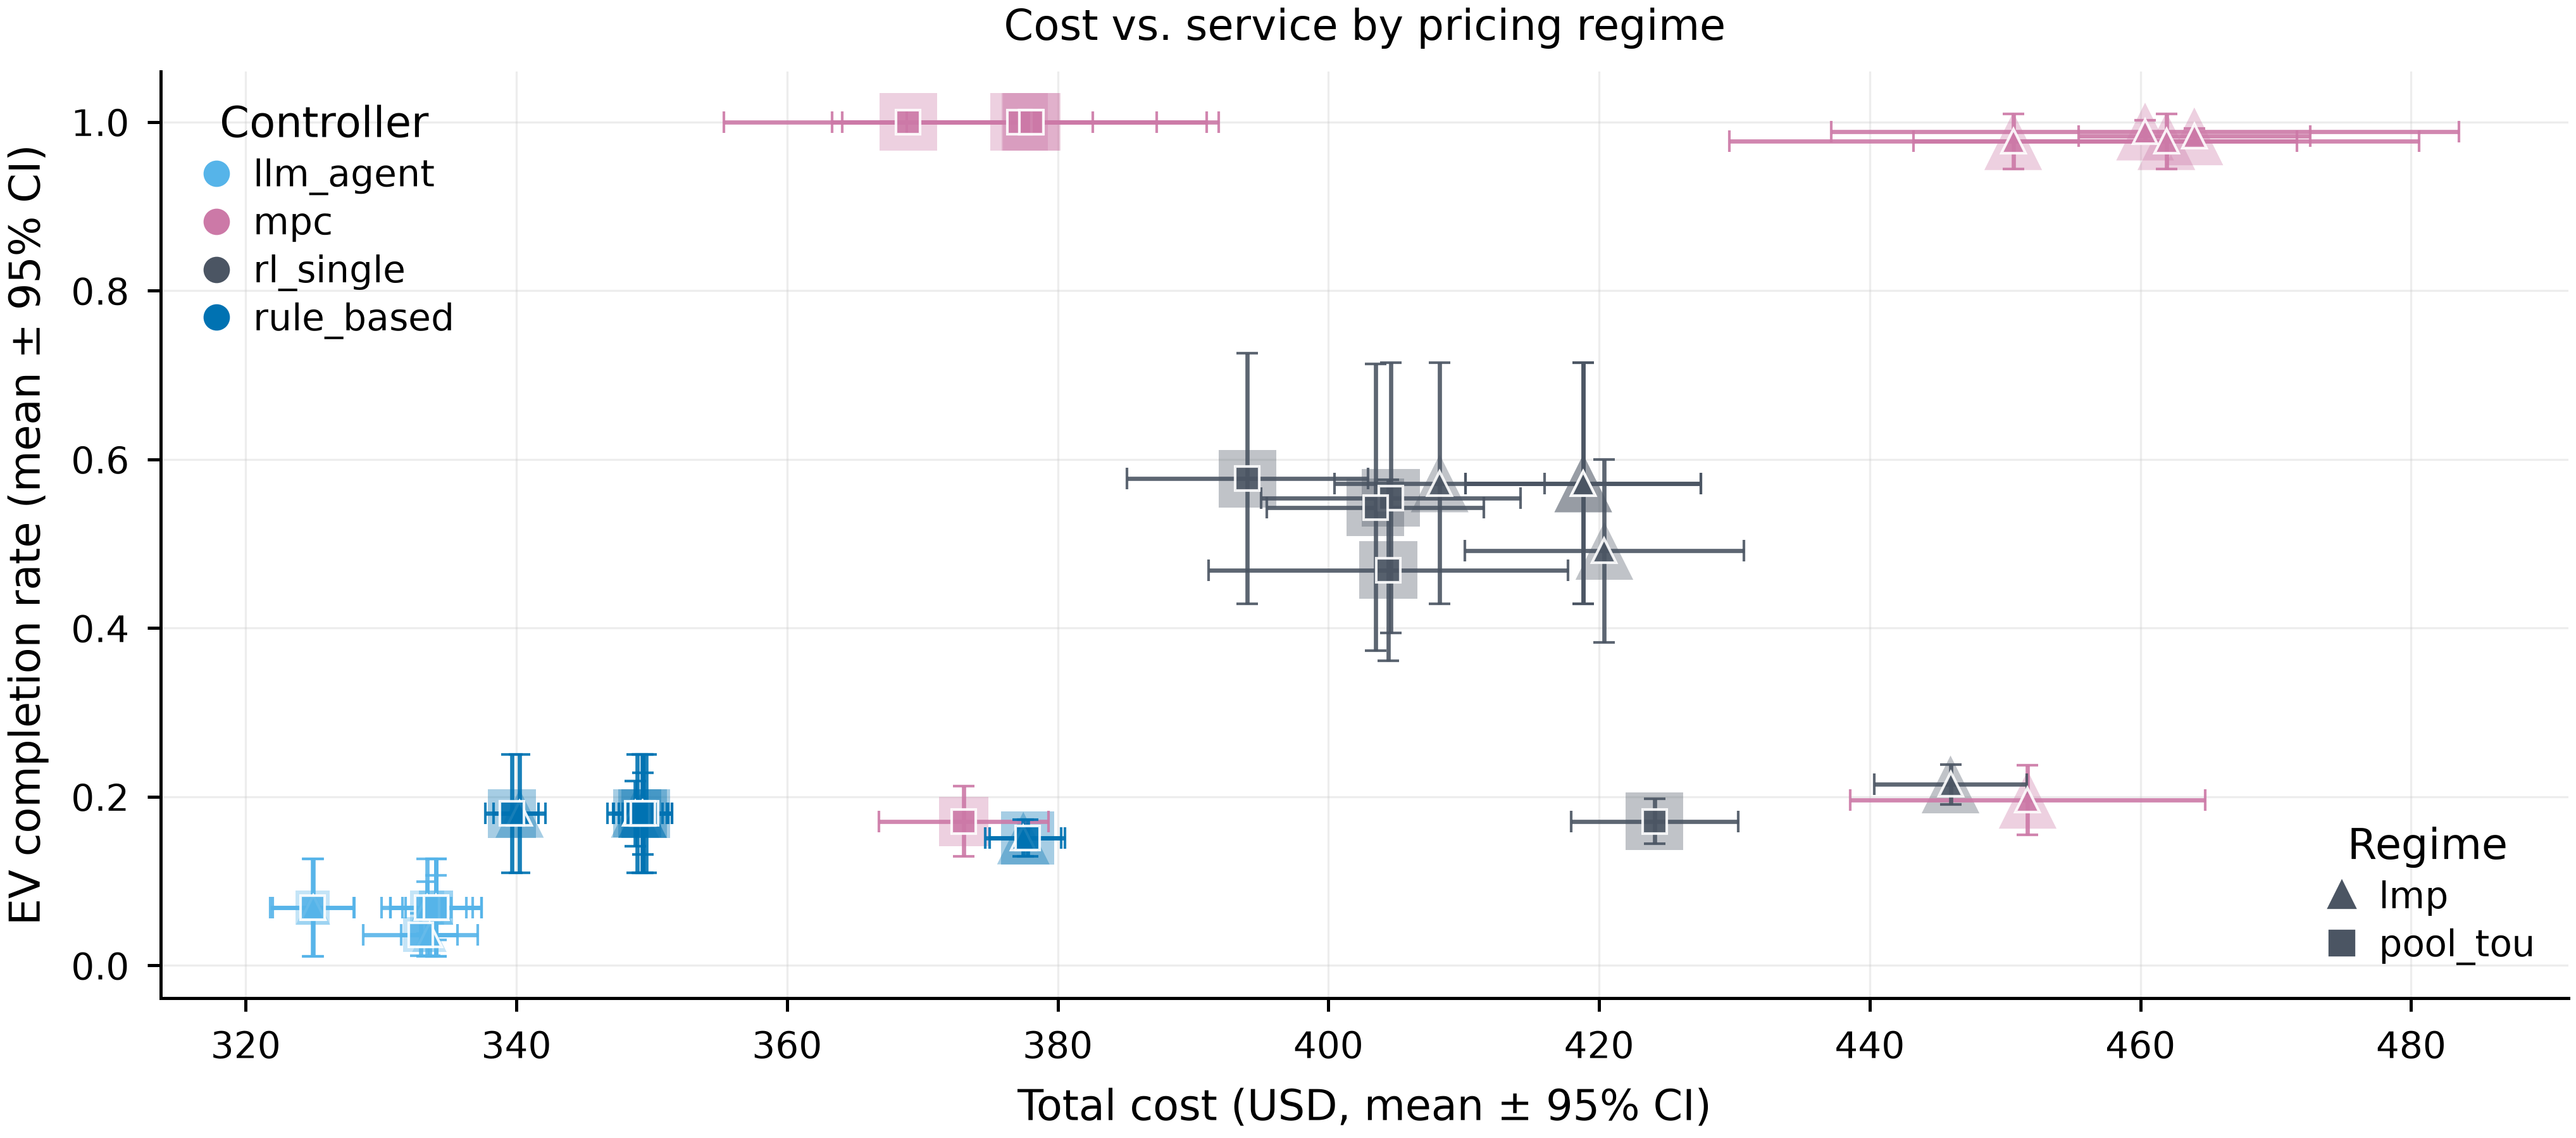
\includegraphics[width=\textwidth]{f7_cost_vs_service}
  \caption{Cost versus EV service across pricing regimes
    (\texttt{pool\_tou} vs.\ \texttt{lmp}): colour denotes the controller,
    marker shape the pricing regime, marker area the mean peak demand, and
    whiskers the 95\% confidence interval over seeds. Each point is one
    (regime, scenario, controller) cell ($N=310$ completed runs).}
  \label{fig:f7-cost-service}
\end{figure*}

% ----------------------------------------------------------------------------
% F8 — locational price dispersal over the week (single column)
%
% NOT EMITTED YET. F8 is gated on the LMP validity guard: a run may only feed
% the dispersal figure when cost_basis == lmp, the price mean is finite and
% positive, the measured spread is non-zero, and there are no OPF fallback
% steps. The current M1 \texttt{lmp} runs are fallback-dominated
% (power_flow_not_converged) with zero/negative measured spread, so drawing a
% "spread" figure now would misrepresent the physics. Uncomment once the guard
% passes and experiments/figures/f8_lmp_dispersal.pdf exists.
% ----------------------------------------------------------------------------
% \begin{figure}[t]
%   \centering
%   \includegraphics[width=\columnwidth]{f8_lmp_dispersal}
%   \caption{Locational marginal price dispersal over the week for the
%     congested scenario: community mean (line) with the min--max band across
%     buildings (shaded). The annotation reports the measured max spread and
%     states explicitly when prices are uniform.}
%   \label{fig:f8-lmp-dispersal}
% \end{figure}

% Requires: \usepackage{graphicx}
%
% Generated by:
%   python -m experiments.paper_figures.make_paper_figures \
%       --runs <runs-root> --out experiments/figures
% <runs-root> layout: <root>/<regime>/<scenario>/<run_id>/result.json
% Figures are vector PDF (fonts embedded) with SVG + 600 dpi PNG previews.
% ACM convention: figure captions go BELOW the figure.
%
% Self-contained: the F7 PDF is committed at paper/figures/. Compile from the
% paper directory (\graphicspath resolves both locations), or drop the PDF next
% to your main .tex.
% ============================================================================

\graphicspath{{figures/}{../experiments/figures/}}

% ----------------------------------------------------------------------------
% F7 — cost vs. service by pricing regime  (full width, two-column layout)
% ----------------------------------------------------------------------------
\begin{figure*}[t]
  \centering
  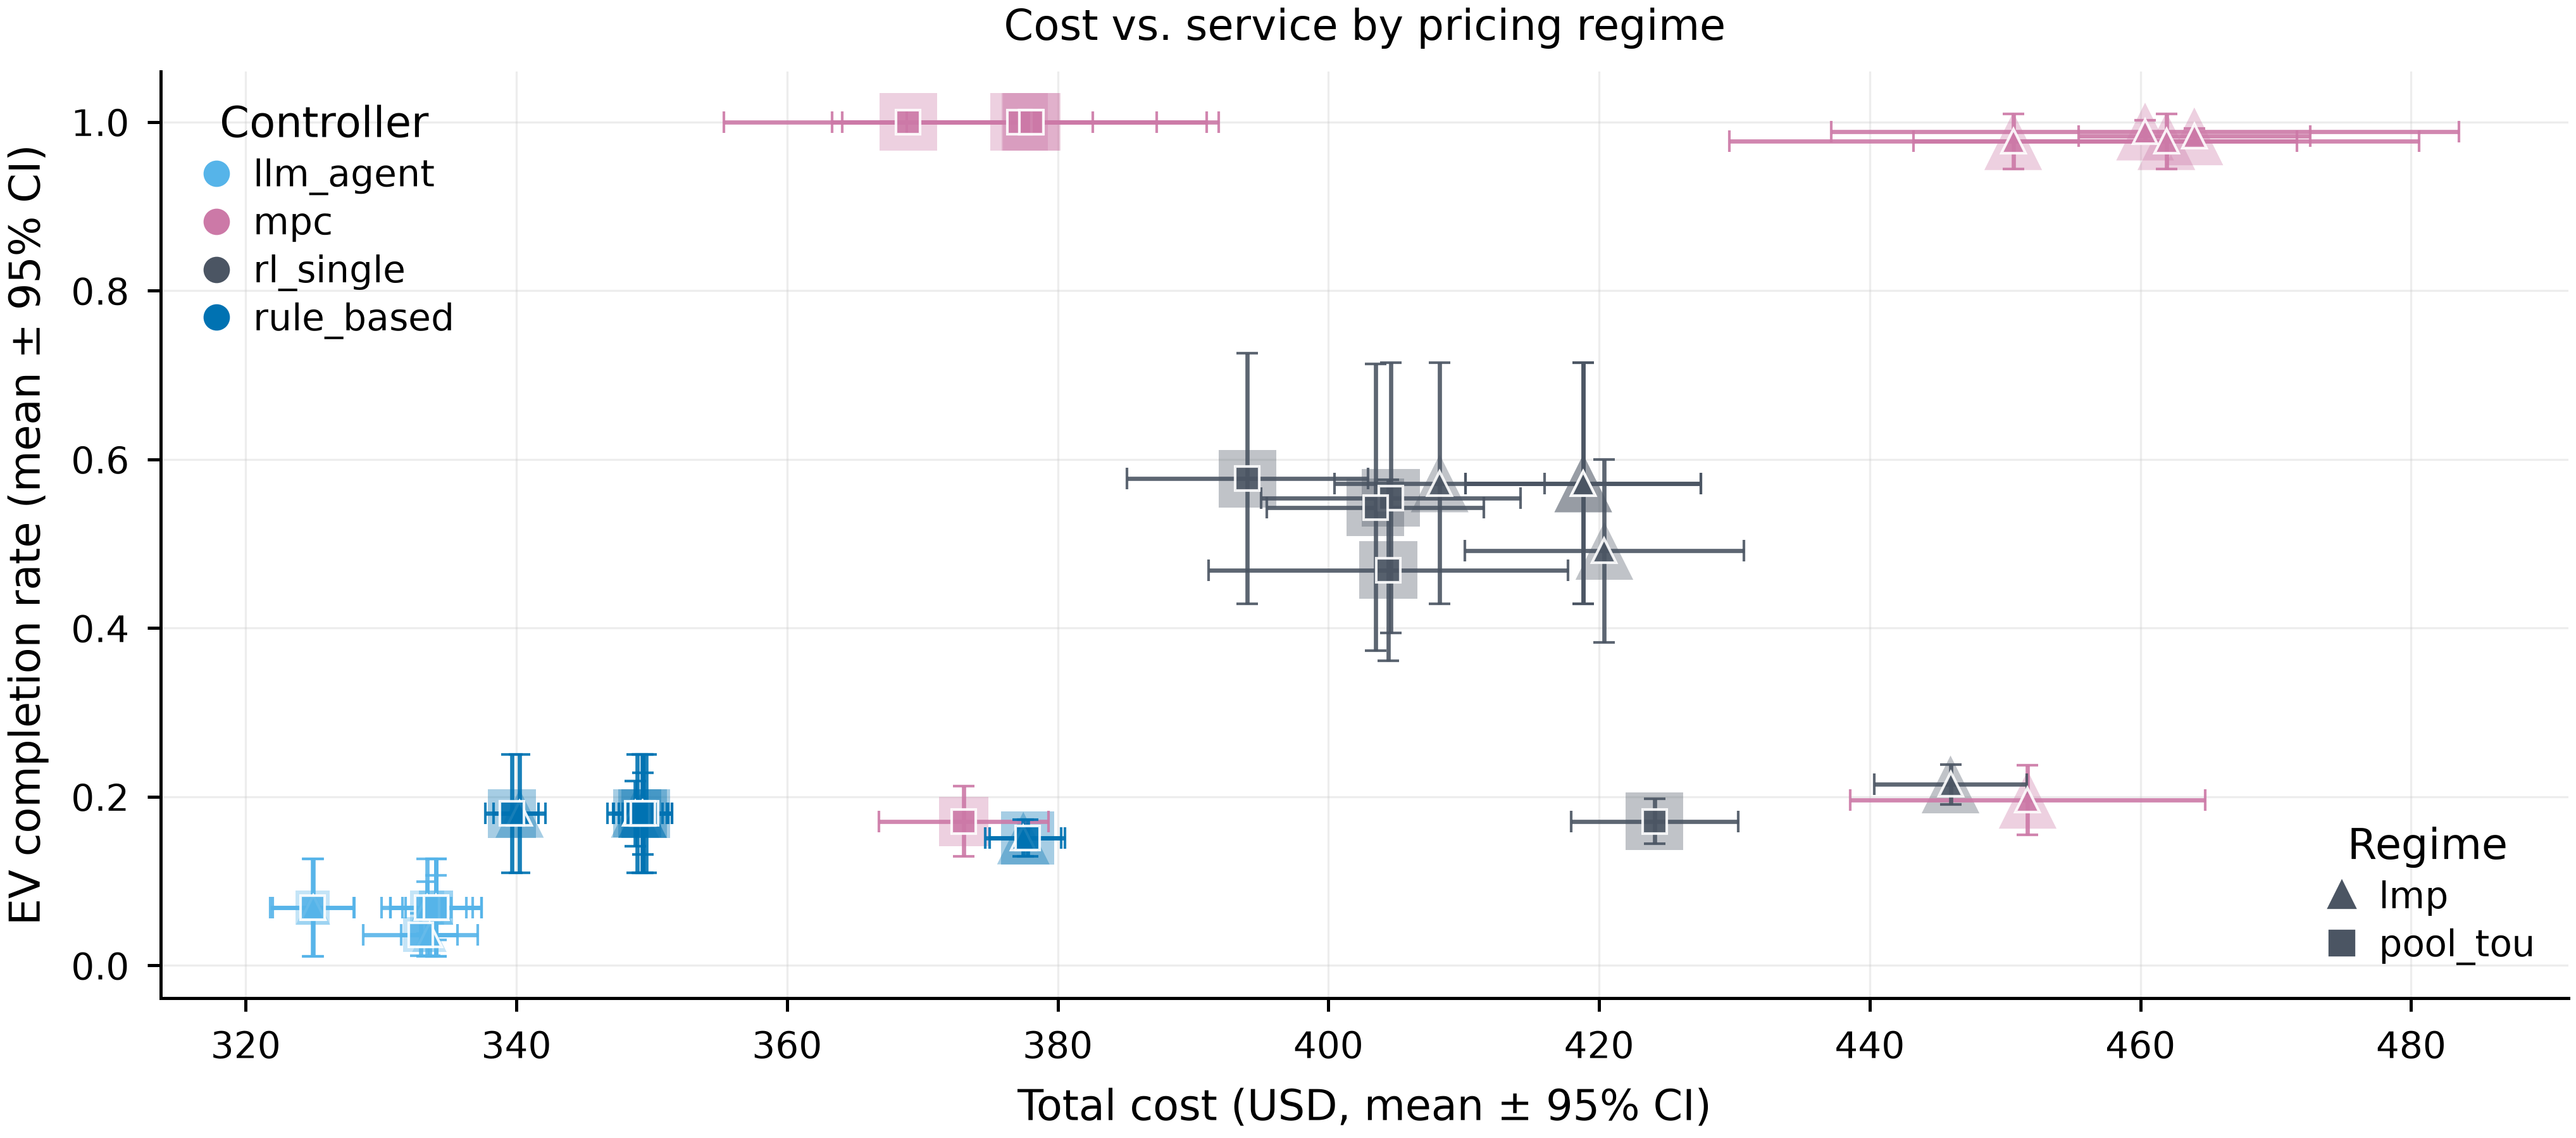
\includegraphics[width=\textwidth]{f7_cost_vs_service}
  \caption{Cost versus EV service across pricing regimes
    (\texttt{pool\_tou} vs.\ \texttt{lmp}): colour denotes the controller,
    marker shape the pricing regime, marker area the mean peak demand, and
    whiskers the 95\% confidence interval over seeds. Each point is one
    (regime, scenario, controller) cell ($N=310$ completed runs).}
  \label{fig:f7-cost-service}
\end{figure*}

% ----------------------------------------------------------------------------
% F8 — locational price dispersal over the week (single column)
%
% NOT EMITTED YET. F8 is gated on the LMP validity guard: a run may only feed
% the dispersal figure when cost_basis == lmp, the price mean is finite and
% positive, the measured spread is non-zero, and there are no OPF fallback
% steps. The current M1 \texttt{lmp} runs are fallback-dominated
% (power_flow_not_converged) with zero/negative measured spread, so drawing a
% "spread" figure now would misrepresent the physics. Uncomment once the guard
% passes and experiments/figures/f8_lmp_dispersal.pdf exists.
% ----------------------------------------------------------------------------
% \begin{figure}[t]
%   \centering
%   \includegraphics[width=\columnwidth]{f8_lmp_dispersal}
%   \caption{Locational marginal price dispersal over the week for the
%     congested scenario: community mean (line) with the min--max band across
%     buildings (shaded). The annotation reports the measured max spread and
%     states explicitly when prices are uniform.}
%   \label{fig:f8-lmp-dispersal}
% \end{figure}

% Requires: \usepackage{graphicx}
%
% Generated by:
%   python -m experiments.paper_figures.make_paper_figures \
%       --runs <runs-root> --out experiments/figures
% <runs-root> layout: <root>/<regime>/<scenario>/<run_id>/result.json
% Figures are vector PDF (fonts embedded) with SVG + 600 dpi PNG previews.
% ACM convention: figure captions go BELOW the figure.
%
% Self-contained: the F7 PDF is committed at paper/figures/. Compile from the
% paper directory (\graphicspath resolves both locations), or drop the PDF next
% to your main .tex.
% ============================================================================

\graphicspath{{figures/}{../experiments/figures/}}

% ----------------------------------------------------------------------------
% F7 — cost vs. service by pricing regime  (full width, two-column layout)
% ----------------------------------------------------------------------------
\begin{figure*}[t]
  \centering
  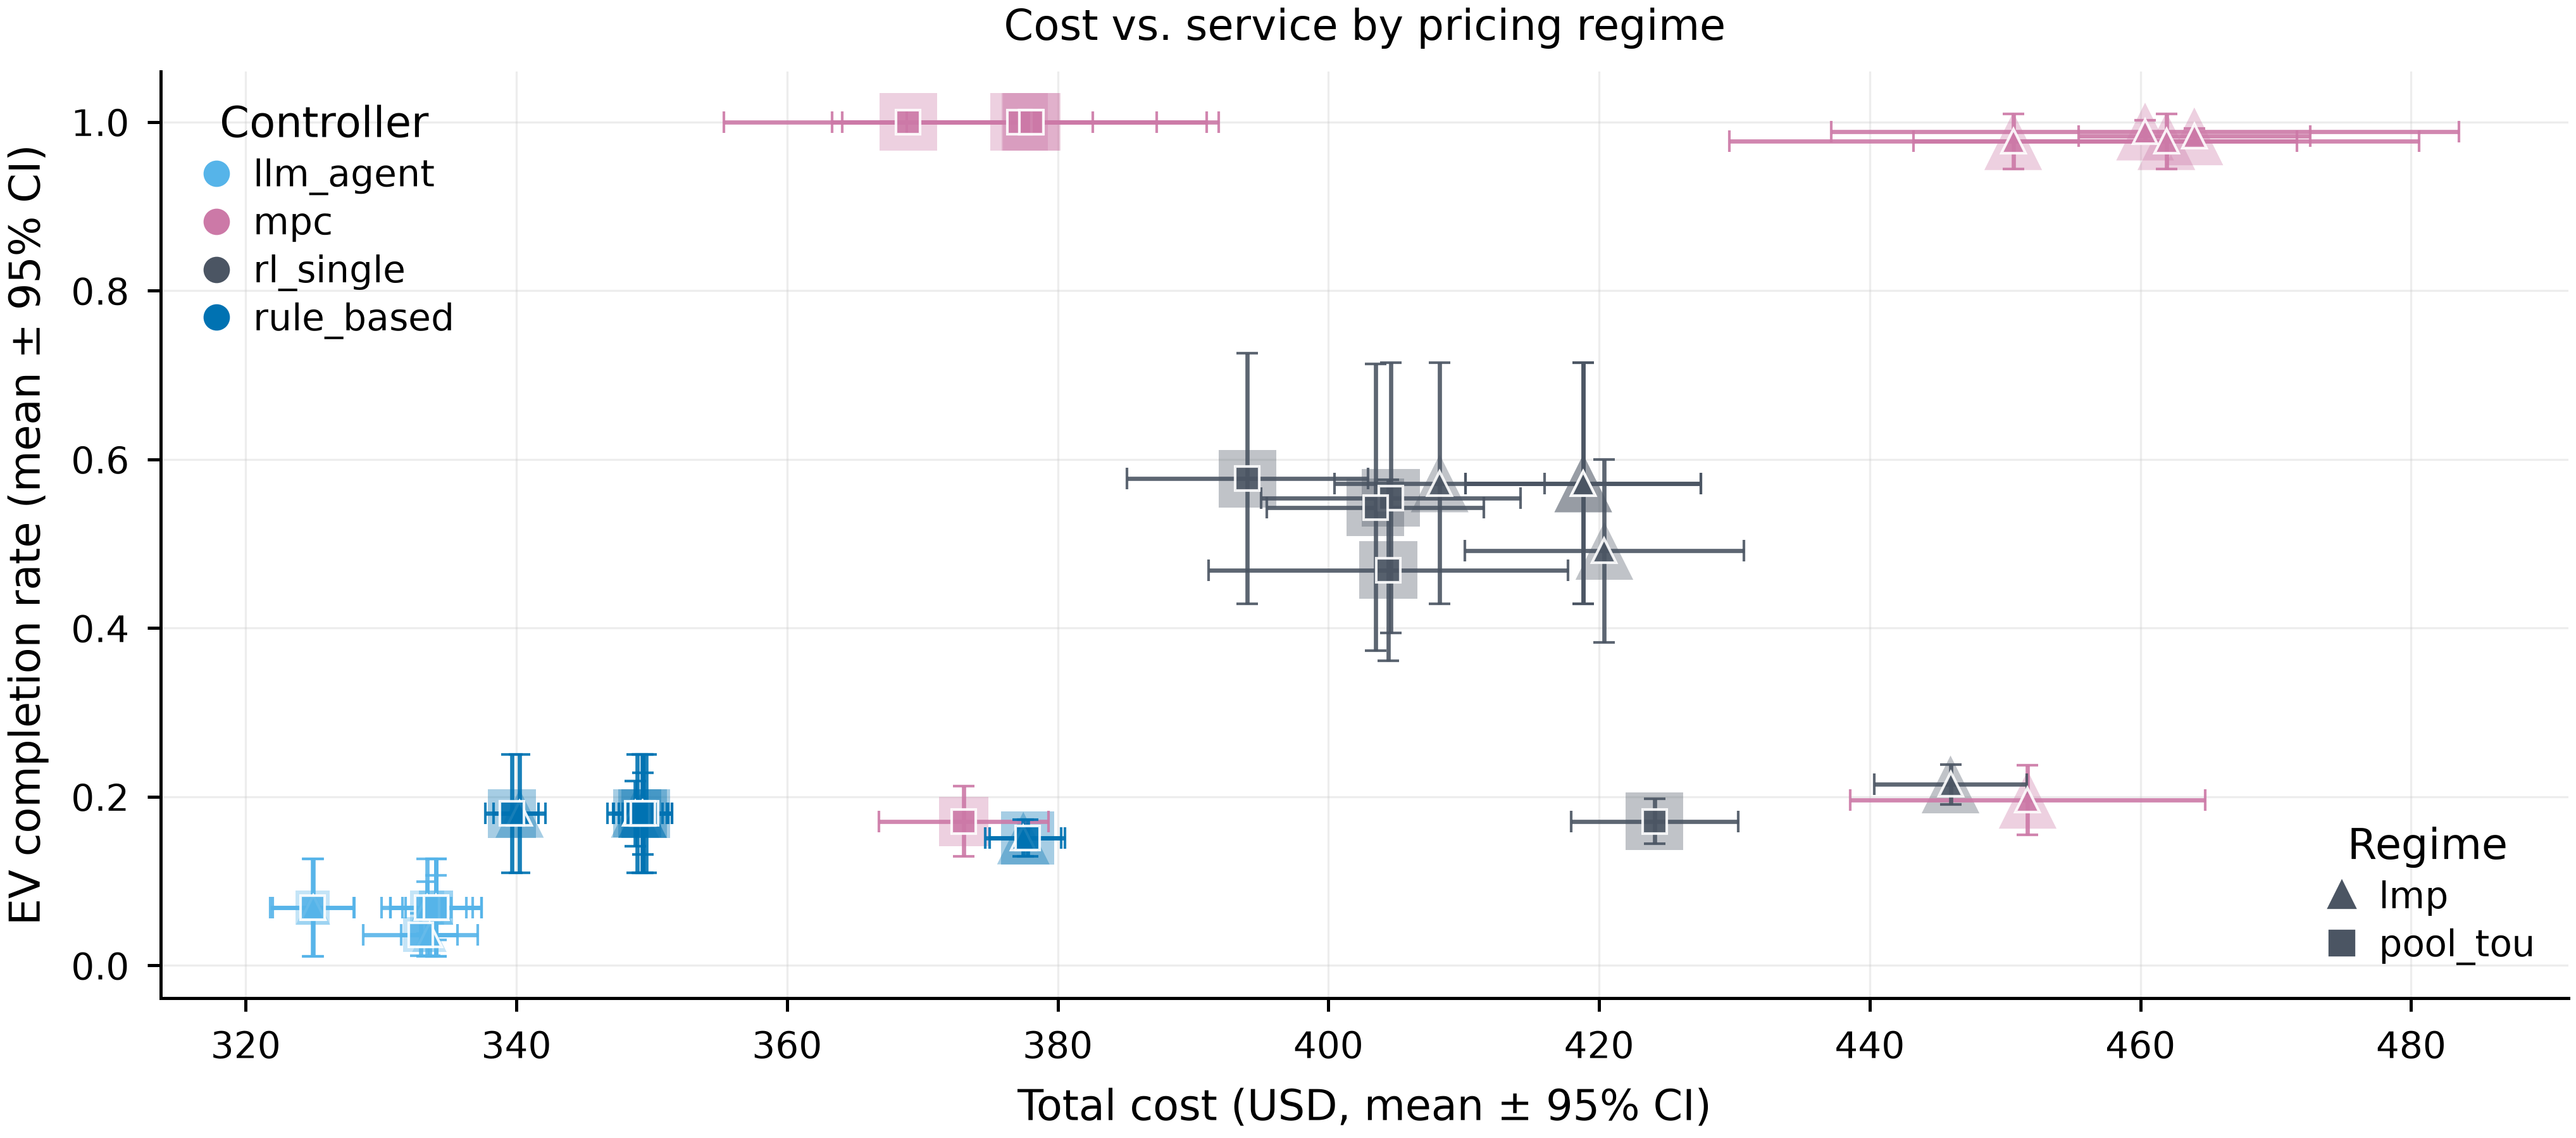
\includegraphics[width=\textwidth]{f7_cost_vs_service}
  \caption{Cost versus EV service across pricing regimes
    (\texttt{pool\_tou} vs.\ \texttt{lmp}): colour denotes the controller,
    marker shape the pricing regime, marker area the mean peak demand, and
    whiskers the 95\% confidence interval over seeds. Each point is one
    (regime, scenario, controller) cell ($N=310$ completed runs).}
  \label{fig:f7-cost-service}
\end{figure*}

% ----------------------------------------------------------------------------
% F8 — locational price dispersal over the week (single column)
%
% NOT EMITTED YET. F8 is gated on the LMP validity guard: a run may only feed
% the dispersal figure when cost_basis == lmp, the price mean is finite and
% positive, the measured spread is non-zero, and there are no OPF fallback
% steps. The current M1 \texttt{lmp} runs are fallback-dominated
% (power_flow_not_converged) with zero/negative measured spread, so drawing a
% "spread" figure now would misrepresent the physics. Uncomment once the guard
% passes and experiments/figures/f8_lmp_dispersal.pdf exists.
% ----------------------------------------------------------------------------
% \begin{figure}[t]
%   \centering
%   \includegraphics[width=\columnwidth]{f8_lmp_dispersal}
%   \caption{Locational marginal price dispersal over the week for the
%     congested scenario: community mean (line) with the min--max band across
%     buildings (shaded). The annotation reports the measured max spread and
%     states explicitly when prices are uniform.}
%   \label{fig:f8-lmp-dispersal}
% \end{figure}

% Requires: \usepackage{graphicx}
%
% Generated by:
%   python -m experiments.paper_figures.make_paper_figures \
%       --runs <runs-root> --out experiments/figures
% <runs-root> layout: <root>/<regime>/<scenario>/<run_id>/result.json
% Figures are vector PDF (fonts embedded) with SVG + 600 dpi PNG previews.
% ACM convention: figure captions go BELOW the figure.
%
% Self-contained: the F7 PDF is committed at paper/figures/. Compile from the
% paper directory (\graphicspath resolves both locations), or drop the PDF next
% to your main .tex.
% ============================================================================

\graphicspath{{figures/}{../experiments/figures/}}

% ----------------------------------------------------------------------------
% F7 — cost vs. service by pricing regime  (full width, two-column layout)
% ----------------------------------------------------------------------------
\begin{figure*}[t]
  \centering
  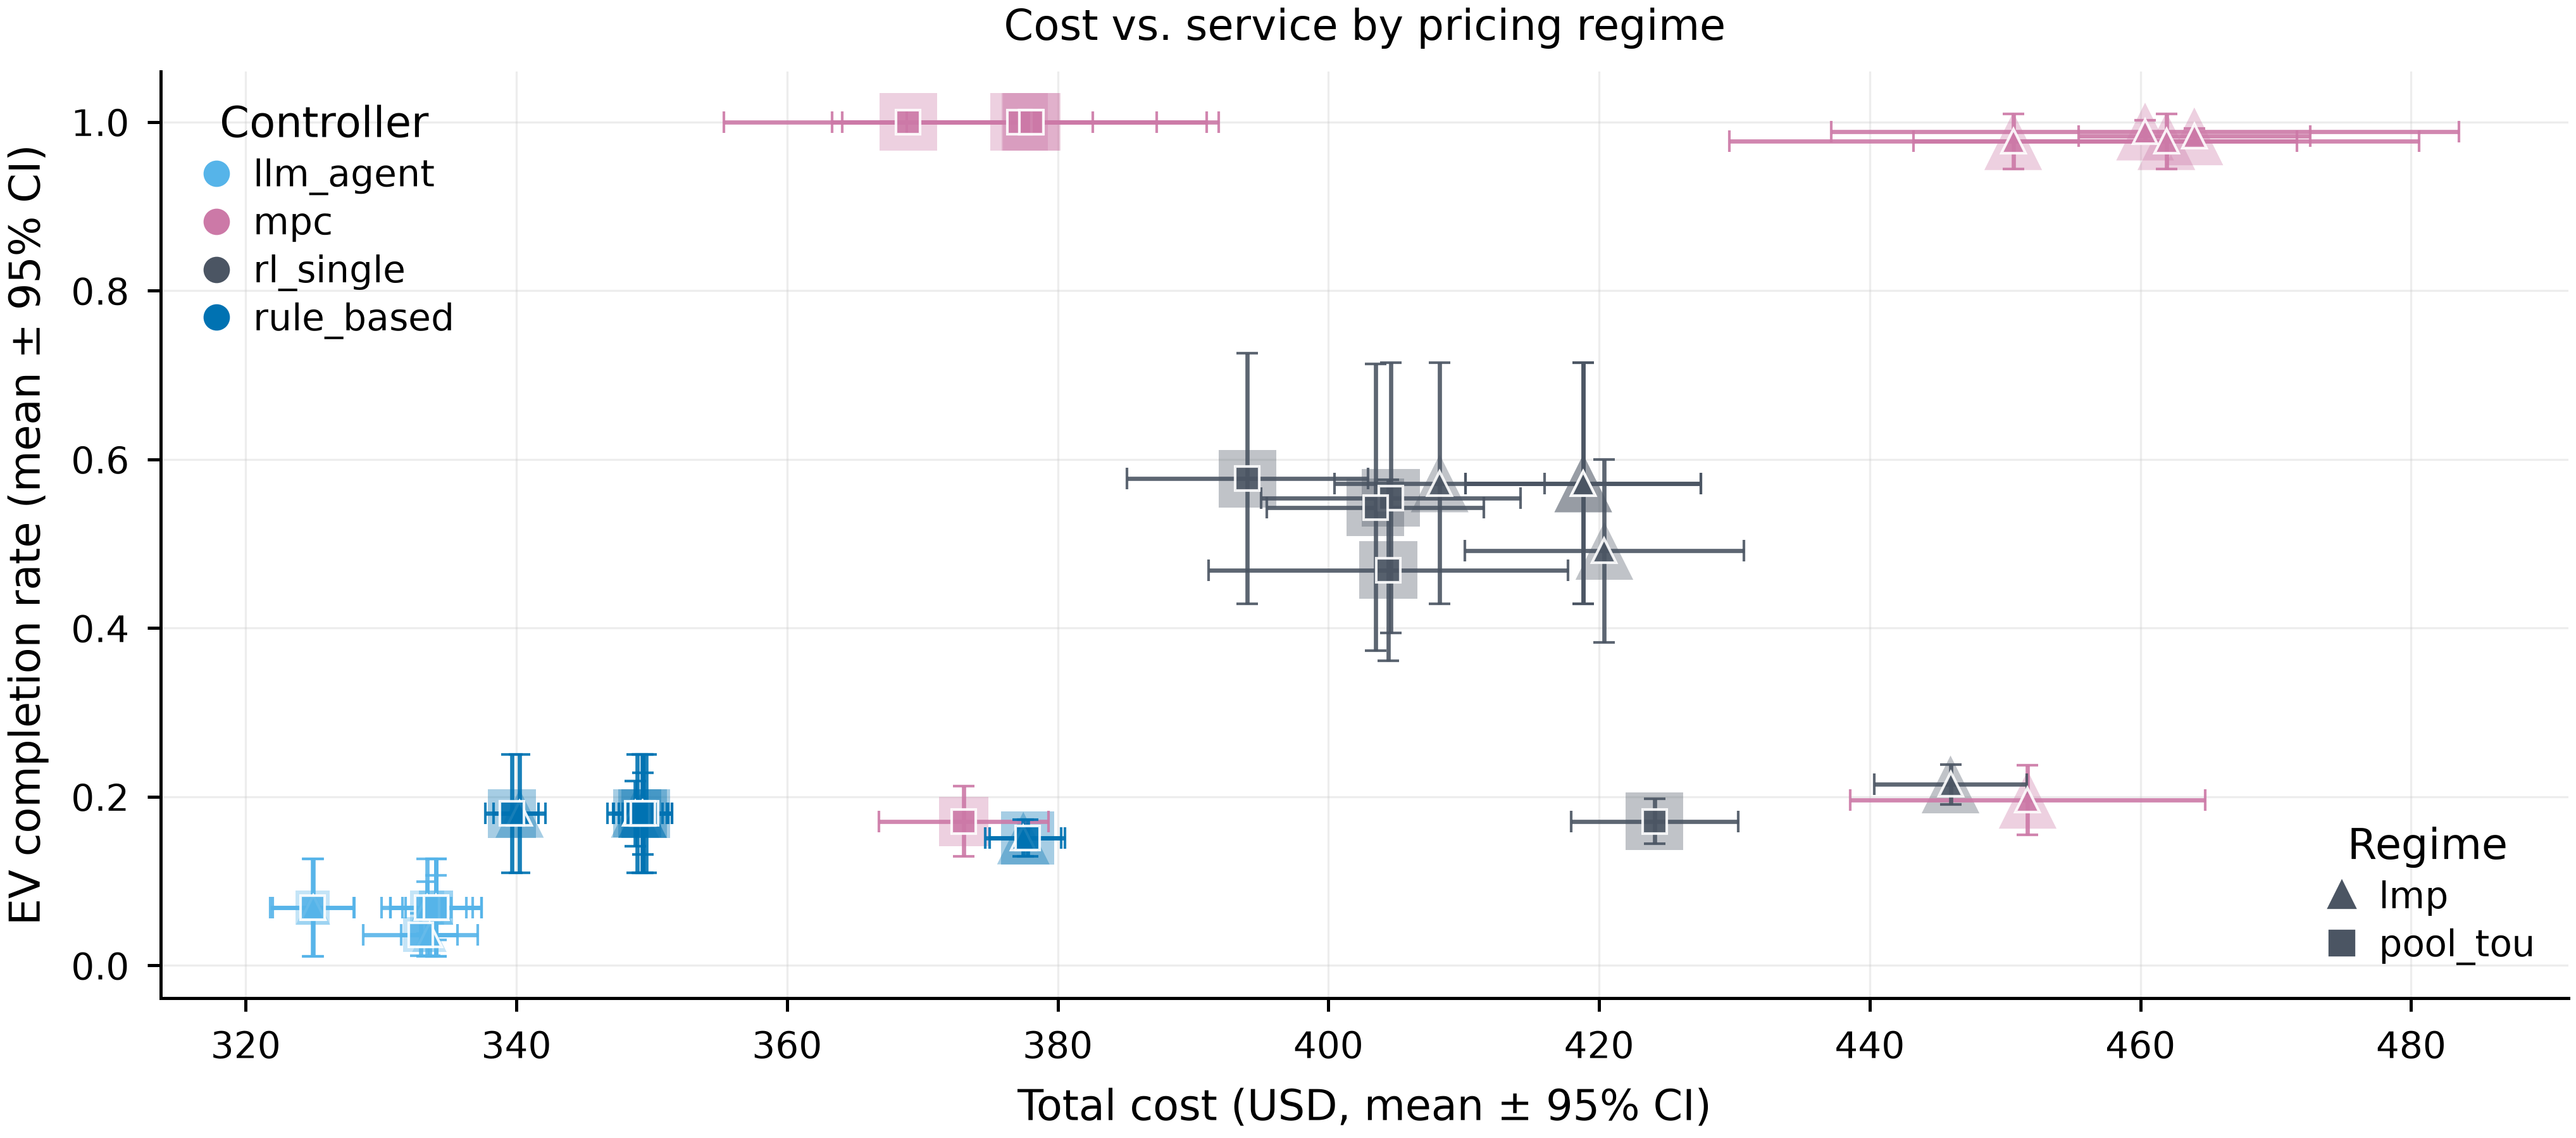
\includegraphics[width=\textwidth]{f7_cost_vs_service}
  \caption{Cost versus EV service across pricing regimes
    (\texttt{pool\_tou} vs.\ \texttt{lmp}): colour denotes the controller,
    marker shape the pricing regime, marker area the mean peak demand, and
    whiskers the 95\% confidence interval over seeds. Each point is one
    (regime, scenario, controller) cell ($N=310$ completed runs).}
  \label{fig:f7-cost-service}
\end{figure*}

% ----------------------------------------------------------------------------
% F8 — locational price dispersal over the week (single column)
%
% NOT EMITTED YET. F8 is gated on the LMP validity guard: a run may only feed
% the dispersal figure when cost_basis == lmp, the price mean is finite and
% positive, the measured spread is non-zero, and there are no OPF fallback
% steps. The current M1 \texttt{lmp} runs are fallback-dominated
% (power_flow_not_converged) with zero/negative measured spread, so drawing a
% "spread" figure now would misrepresent the physics. Uncomment once the guard
% passes and experiments/figures/f8_lmp_dispersal.pdf exists.
% ----------------------------------------------------------------------------
% \begin{figure}[t]
%   \centering
%   \includegraphics[width=\columnwidth]{f8_lmp_dispersal}
%   \caption{Locational marginal price dispersal over the week for the
%     congested scenario: community mean (line) with the min--max band across
%     buildings (shaded). The annotation reports the measured max spread and
%     states explicitly when prices are uniform.}
%   \label{fig:f8-lmp-dispersal}
% \end{figure}
